\documentclass[12pt]{report}
\setlength{\textwidth}{6.5 in}
\setlength{\evensidemargin}{0 in}
\setlength{\oddsidemargin}{0 in}
\setlength{\textheight}{9.4 in }
\setlength{\topmargin}{-0.7 in}
\pagestyle{myheadings}
\usepackage[pdftex]{graphicx} \usepackage{eso-pic}
\usepackage{amsmath}
\usepackage{amssymb}
\usepackage{graphicx}
\usepackage{placeins}
\usepackage{ifthen}
\usepackage{tikz}
\usepackage{pgfplots}
\usepackage{array}  % for table column M
\usepackage{makecell} % to break line within a cell
\usepackage{verbatim}
\usepackage{epstopdf}
\usepackage{amsfonts}
\usepackage{xcolor}
\usepackage{subcaption}
\usepackage{pdfpages}
\usepackage{hyperref}
%\captionsetup{compatibility=false}
%\usepackage{dsfont}
\usepackage[absolute,overlay]{textpos}
\usetikzlibrary{calc, angles,quotes}
\usetikzlibrary{pgfplots.fillbetween, backgrounds}
\usetikzlibrary{positioning}
\usetikzlibrary{arrows}
\usetikzlibrary{pgfplots.groupplots}
\usetikzlibrary{arrows.meta}
\usetikzlibrary{plotmarks}
\usetikzlibrary{decorations.markings}

\DeclareGraphicsExtensions{.pdf,.eps,.png}

\definecolor{matlabcomment}{RGB}{34,139,34}

\pgfmathdeclarefunction{gauss}{1}{%
	\pgfmathparse{1/(sqrt(2*pi))*exp(-((#1)^2)/2)}%
}

\pgfmathdeclarefunction{laplacian}{2}{%
	\pgfmathparse{1/(#2*2)*exp(-(abs(x-#1))/(#2))}%
}

\pgfmathdeclarefunction{pretty_func}{1}{%
	\pgfmathparse{cos(deg(#1/2)) - sin(deg(#1)) + cos(deg(#1/2)-45) - sin(deg(#1/4)-154)}%
}

\pgfplotsset{
	dirac/.style={
		mark=triangle*,
		mark options={scale=2},
		ycomb,
		scatter,
		visualization depends on={y/abs(y)-1 \as \sign},
		scatter/@pre marker code/.code={\scope[rotate=90*\sign,yshift=-2pt]}
	}
}

\def\thickness{very thick}

\tikzset{
amark/.style 2 args={
	decoration={             
		markings, 
		mark=at position {0.5} with { 
			\arrow{stealth},
			\node[#2] {#1};
		}
	}, \thickness,
	postaction={decorate}
},
earlymark/.style 2 args={
	decoration={             
		markings, 
		mark=at position {0.25} with { 
			\arrow{stealth},
			\node[#2] {#1};
		}
	}, \thickness,
	postaction={decorate}
},
latemark/.style 2 args={
	decoration={             
		markings, 
		mark=at position {0.8} with { 
			\arrow{stealth},
			\node[#2] {#1};
		}
	}, \thickness,
	postaction={decorate}
},
zpath/.style={
	decoration={             
		markings, 
		mark=at position {0.5} with { 
			\arrow{stealth},
			\node[#1] {$z^{-1}$};
		}
	}, \thickness,
	postaction={decorate}
},
terminal/.style 2 args={draw,circle,inner sep=2pt,label={#1:#2}},
}


\tikzset{
	invisible/.style={opacity=0},
	visible on/.style={alt={#1{}{invisible}}},
	alt/.code args={<#1>#2#3}{%
		\alt<#1>{\pgfkeysalso{#2}}{\pgfkeysalso{#3}} % \pgfkeysalso doesn't change the path
	},
}

\newcommand\PlotSampledSpectrum[4]{%
	\def\fs{#2}%
	\def\fmax{#3}%
	\def\ros{#4}%
	\input{#1}%
}

\pgfmathdeclarefunction{invgauss}{2}{%
	\pgfmathparse{sqrt(-2*ln(#1))*cos(deg(2*pi*#2))}%
}

\tikzset{
	declare function={
		sinc(\x) = (and(\x!=0, 1) * (sin(deg(pi*\x))/(pi*\x)) +
		(and(\x==0, 1) * 1);
	}
}

\DeclareMathOperator{\E}{\mathbb{E}} % expectation

\newcommand\SimpleSys[4]{%
	\def\xin{#2}%
	\def\Hz{#3}%
	\def\yout{#4}
	\input{#1}%
}

\markboth{\em EE264: Homework \#06}{\em EE264: Homework \#06}

\begin{document}
\thispagestyle{empty}
\begin{centering}
	{\large Stanford University}\\
	{\large EE 264: Digital Signal Processing}\\
	{\large Summer, 2018} \\
	\mbox{}\\
	{\large Homework \#06}\\
	\mbox{}\\
\end{centering}
\noindent Date assigned:  August 6, 2018 \hfill
Date due: August 15, 2018\\
\noindent \rule{6.5 in}{0.5pt}
%\mbox{}\\
\noindent {\bf Reading:}  This assignment covers primarily lectures 10 to 12, which correspond to chapters 8, and 10 of the textbook {\bf DTSP 3e}. \\
\noindent {\bf Homework submission:}  Please submit your solutions on Gradescope. Create a single .pdf file containing all your analytical derivations, sketches, plots, and Matlab code (if applicable). \\
\noindent {\bf Extensions and late submissions:}  To ensure that we can release the solutions of this assignment in a timely manner for the final exam, we \underline{cannot} grant extensions or accept late submissions.

\noindent
\rule{6.5 in}{0.5pt}
\mbox{}\\

\noindent {\bf Problem 1: Adapted from the final exam of EE 373A -- Winter 2018 (40 points)}

\noindent \textbf{General description}

As discussed in class, we can use adaptive filters to cancel noise or interference from a desired signal by appropriately filtering a correlated noise measurement. In this exercise, you will build a typical noise canceling system to minimize the noise from an audio signal. Figure~\ref{fig:noise-gen} shows the diagram of noise generation. The speaker produces a signal $s[n]$, like a song, for instance. Only the front microphone captures the signal produced by the speaker. But both microphones capture the noise generated by a noise source. The transfer function $H(z)$ is unknown, and it relates the noise in the rear microphone to the noise in the front microphone. To keep things simple, we will assume that this transfer function is linear and time invariant.

\begin{figure}[!h]
	\centering
	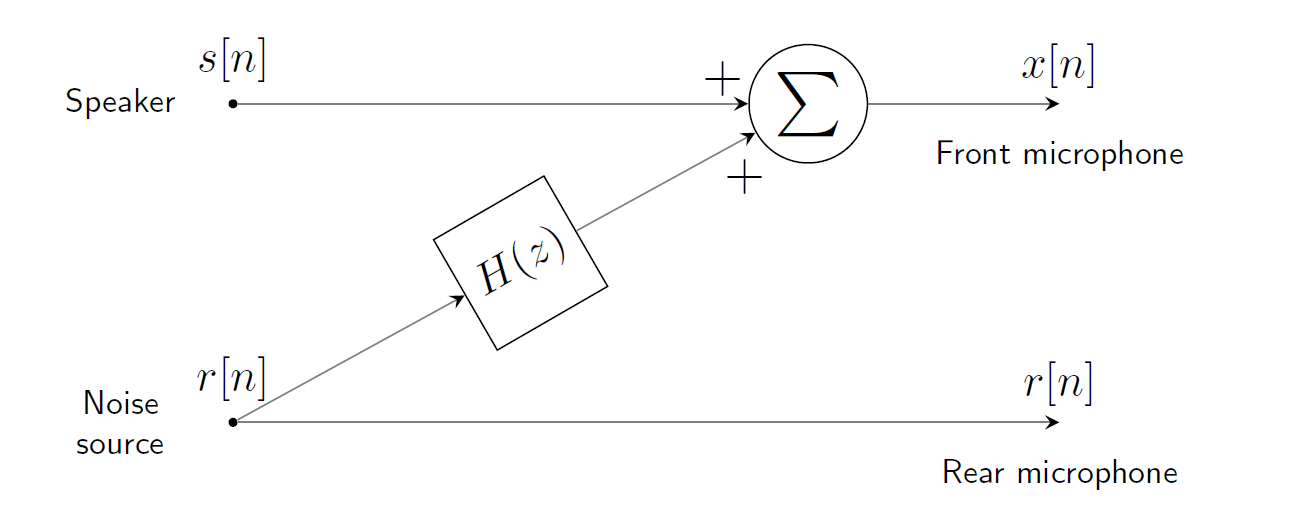
\includegraphics[width=0.6\textwidth]{figs/noise_generation.png}
	\caption{Model for noise generation.} \label{fig:noise-gen}
\end{figure}

The adaptive noise canceler is shown in Figure~\ref{fig:noise-cancel}. The noise from the rear microphone is filtered by the adaptive filter and added to the signal captured by the front microphone. Ideally, the signal $y[n]$ would perfectly cancel the noise component of $x[n]$.

\begin{figure}[!h]
	\centering
	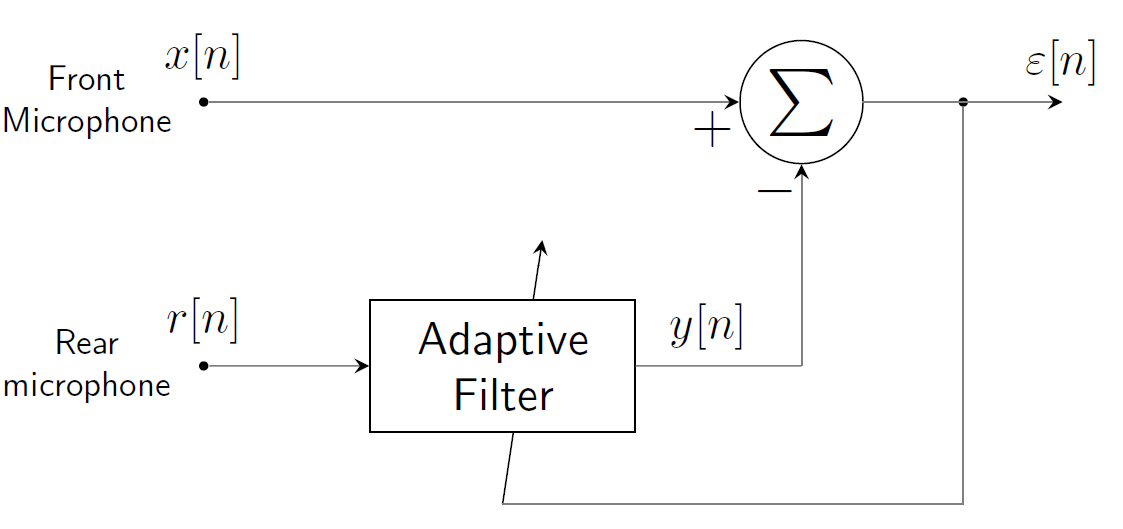
\includegraphics[width=0.6\textwidth]{figs/noise_cancelling.png}
	\caption{Typical noise canceling system.} \label{fig:noise-cancel}
\end{figure}

You're given the audio signal $s[n]$ in the file \texttt{guitartune.wav}. $H(z)$ is given in the file \texttt{problem1\_template.m}. The noise $r[n]$ is a white, zero-mean Gaussian noise with variance $\sigma^2_r = 2\times 10^{-3}$. This value
of variance is chosen so that the signal-to-noise ratio (SNR) at the front microphone is approximately 10 in linear units (or 10 dB). Assume that the adaptive filter has a total 50 weights. To generate the corrupted signal at the front microphone $x[n]$ follow the diagram of Figure~\ref{fig:noise-gen}.

Based on the given information, please answer the following questions. You may use the
Matlab file \texttt{problem1\_template.m}. as a template to develop your answers. This file also contains some useful Matlab hints. Please include your code in your solutions file.

\begin{description}
	\item [(a)] Give an expression for the transfer function of the adaptive filter that would result in perfect noise cancellation. Your answer should depend on $H(z)$ only.
	\item [(b)] What is the Wiener solution for the weights of the adaptive filter if $x[n]$ and $r[n]$ were uncorrelated? In other words, what would be the resulting adaptive filter if there were noise component in $x[n]$?
	\item [(c)] Calculate the adaptation constant $\mu$ such that $\mu = 0.001\mu_{max}$, where $\mu_{max} = 1/\mathrm{trace}(R)$.
	\item [(d)] Using the value of $\mu$ you computed in part (c), estimate how long it takes, in seconds, for the LMS algorithm to converge. You may assume that convergence is achieved after 4 time constants. The sampling frequency of the audio signal is 22.05 kHz. 
	\item [(d)] Describe whether the following metrics would increase, decrease, or remain the same, if we increase the value of $\mu$. Please justify your answers with one or two sentences.
	\begin{itemize}
		\item Convergence time (learning curve time constants)
		\item Minimum mean square error ($\xi_{min}$)
		\item Excess mean square error
	\end{itemize}
	\item [(e)] Implement the adaptive noise canceling system shown in Figure~\ref{fig:noise-cancel}. In addition to your code, turn in the following plots: 
	\begin{itemize}
		\item The mean square noise $(s[n] - \varepsilon[n])^2$ averaged over 20 independent runs. The $x$-axis of your plot should be time in seconds.
		\item On a separate graph, plot the coefficients of the converged adaptive filter you obtained at the last iteration of the last run.
		\item On another graph, plot the magnitude and phase response of the converged adaptive filter. Compare it to the magnitude and phase response of the ideal noise canceler you proposed in part (a). Explain any discrepancies.
	\end{itemize}

	Use the Matlab function \texttt{sound} to play the input signal to the noise canceler $x[n]$, and the noise-canceled signal $\varepsilon[n]$. For the latter, you should be able to hear the noise progressively becoming smaller.
	
	\textit{Matlab hint:} the Matlab functions \texttt{impz} and \texttt{freqz} are useful for plotting impulse response, and magnitude and phase responses of discrete-time systems.
	
\end{description}

\noindent {\bf Problem 2: DFTs of simple sequences (20 points)} 

Given these 8-point signals $x[n], n = 0, \ldots, 7$, compute the 8-point DFTs of $X[k], n = 0, \ldots, 7$. Only \underline{minimal computation} should be required. For example, once you find the answer for (a), you can use DFT properties to find the answers for (b), (c) and (d). Similarly, once you find the answer for (e), you can easily find the answer for (f).

\begin{description}
	\item [(a)] $x[n] = \{1, 1, 1, 1, 1, 1, 1, 1\}$
	\item [(b)] $x[n] = \{1, -1, 1, -1, 1, -1, 1, -1\}$
	\item [(c)] $x[n] = e^{j\pi/2 n}, n = 0, \ldots, 7$
	\item [(d)] $x[n] = \sin(\pi n/2), n = 0, \ldots, 7$
	\item [(e)] $x[n] = \{1, 0, 0, 0, 0, 0, 0, 0\}$
	\item [(f)] $x[n] = \{0, 0, 1, 0, 0, 0, 0, 0\}$
\end{description}

\newpage
\noindent {\bf Problem 3: DFTs (15 points)} 

Consider the six real signals $x_1[n], \ldots, x_6[n]$ shown in Figure~\ref{fig:sequences}, and the six DFTs $X_a[k], \ldots, X_f[k]$ shown in Figure~\ref{fig:dfts}, each of length $N = 8$. Match each signal to its DFT. Provide a table like the following, filling the appropriate letters in the second column. Provide a brief justification based on symmetry, slope of the phase  $\angle X[n]$, d.c. value $X[0]$, etc. 

\noindent\textit{Hint:} aside from looking at the table of DFT properties, you may find it helpful to think about the periodic extension $\tilde{x}[n]$ of each $x[n]$.


\begin{center}
	\begin{tabular}{c|c|p{10cm}}
	Signal & DFT & Justification \\
	\hline
	1 & & \\
	2 & & \\
	3 & & \\
	4 & & \\
	5 & & \\
	6 & & \\
	\hline
\end{tabular}
\end{center}

\FloatBarrier
\begin{figure}[h!]
	\centering
	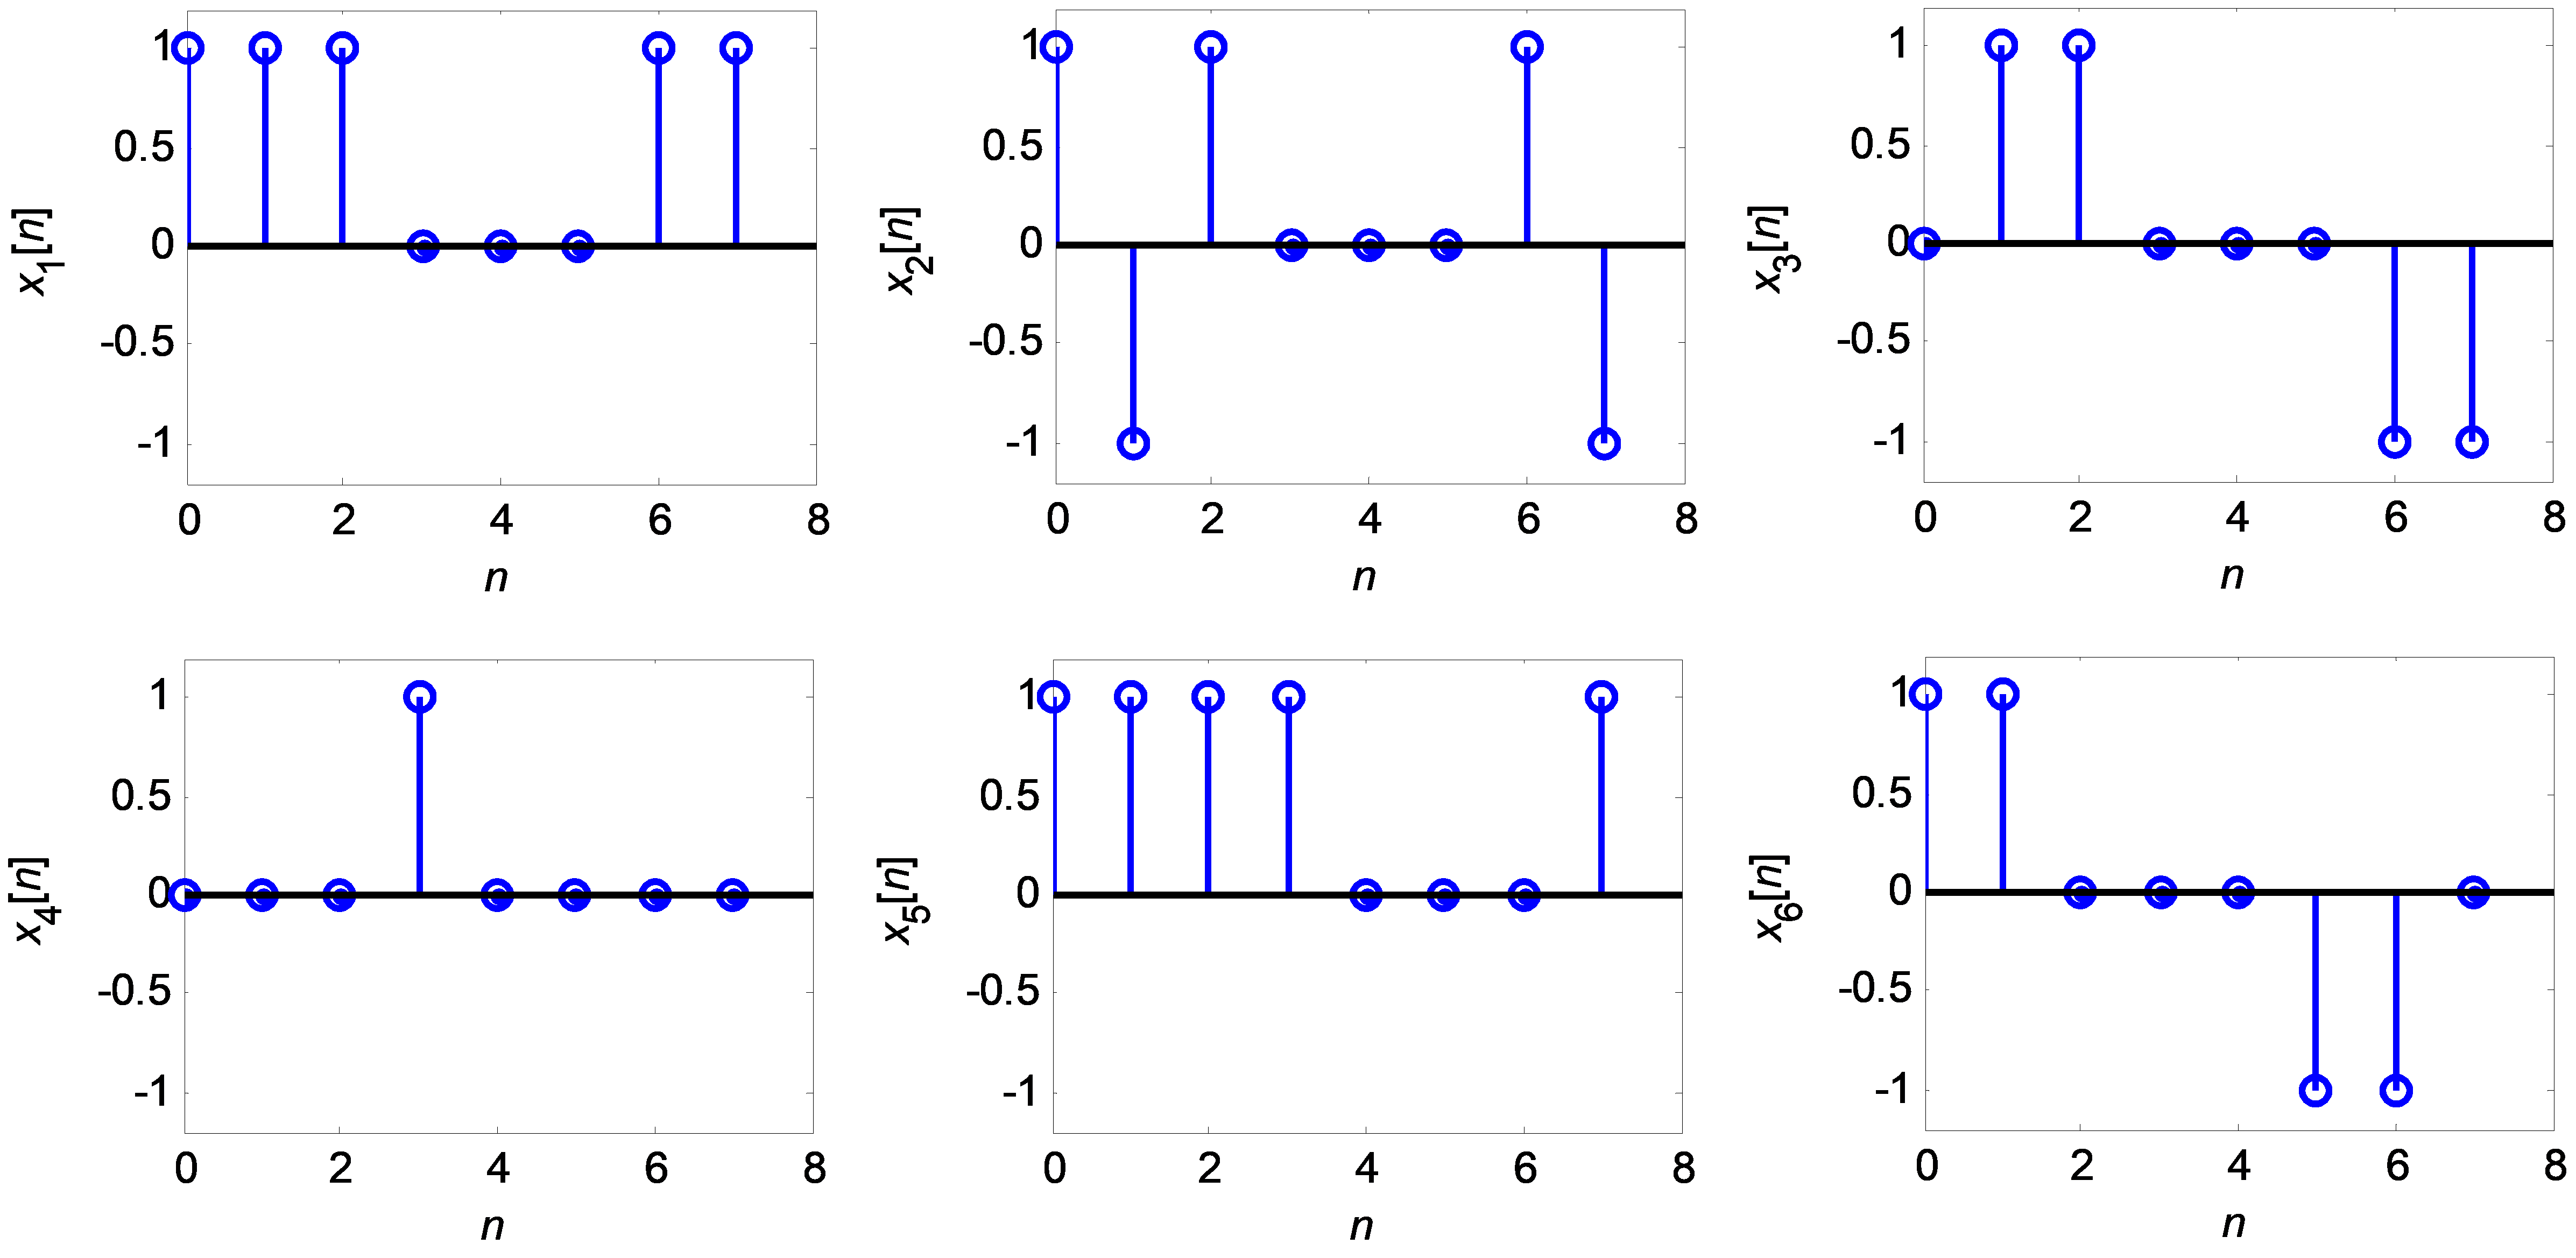
\includegraphics[width=\textwidth]{figs/signals_match_dft.png}
	\caption{8-point real signals $x_1[n], \ldots, x_6[n]$}
	\label{fig:sequences}
\end{figure}
\FloatBarrier

\FloatBarrier
\begin{figure}[h!]
	\centering
	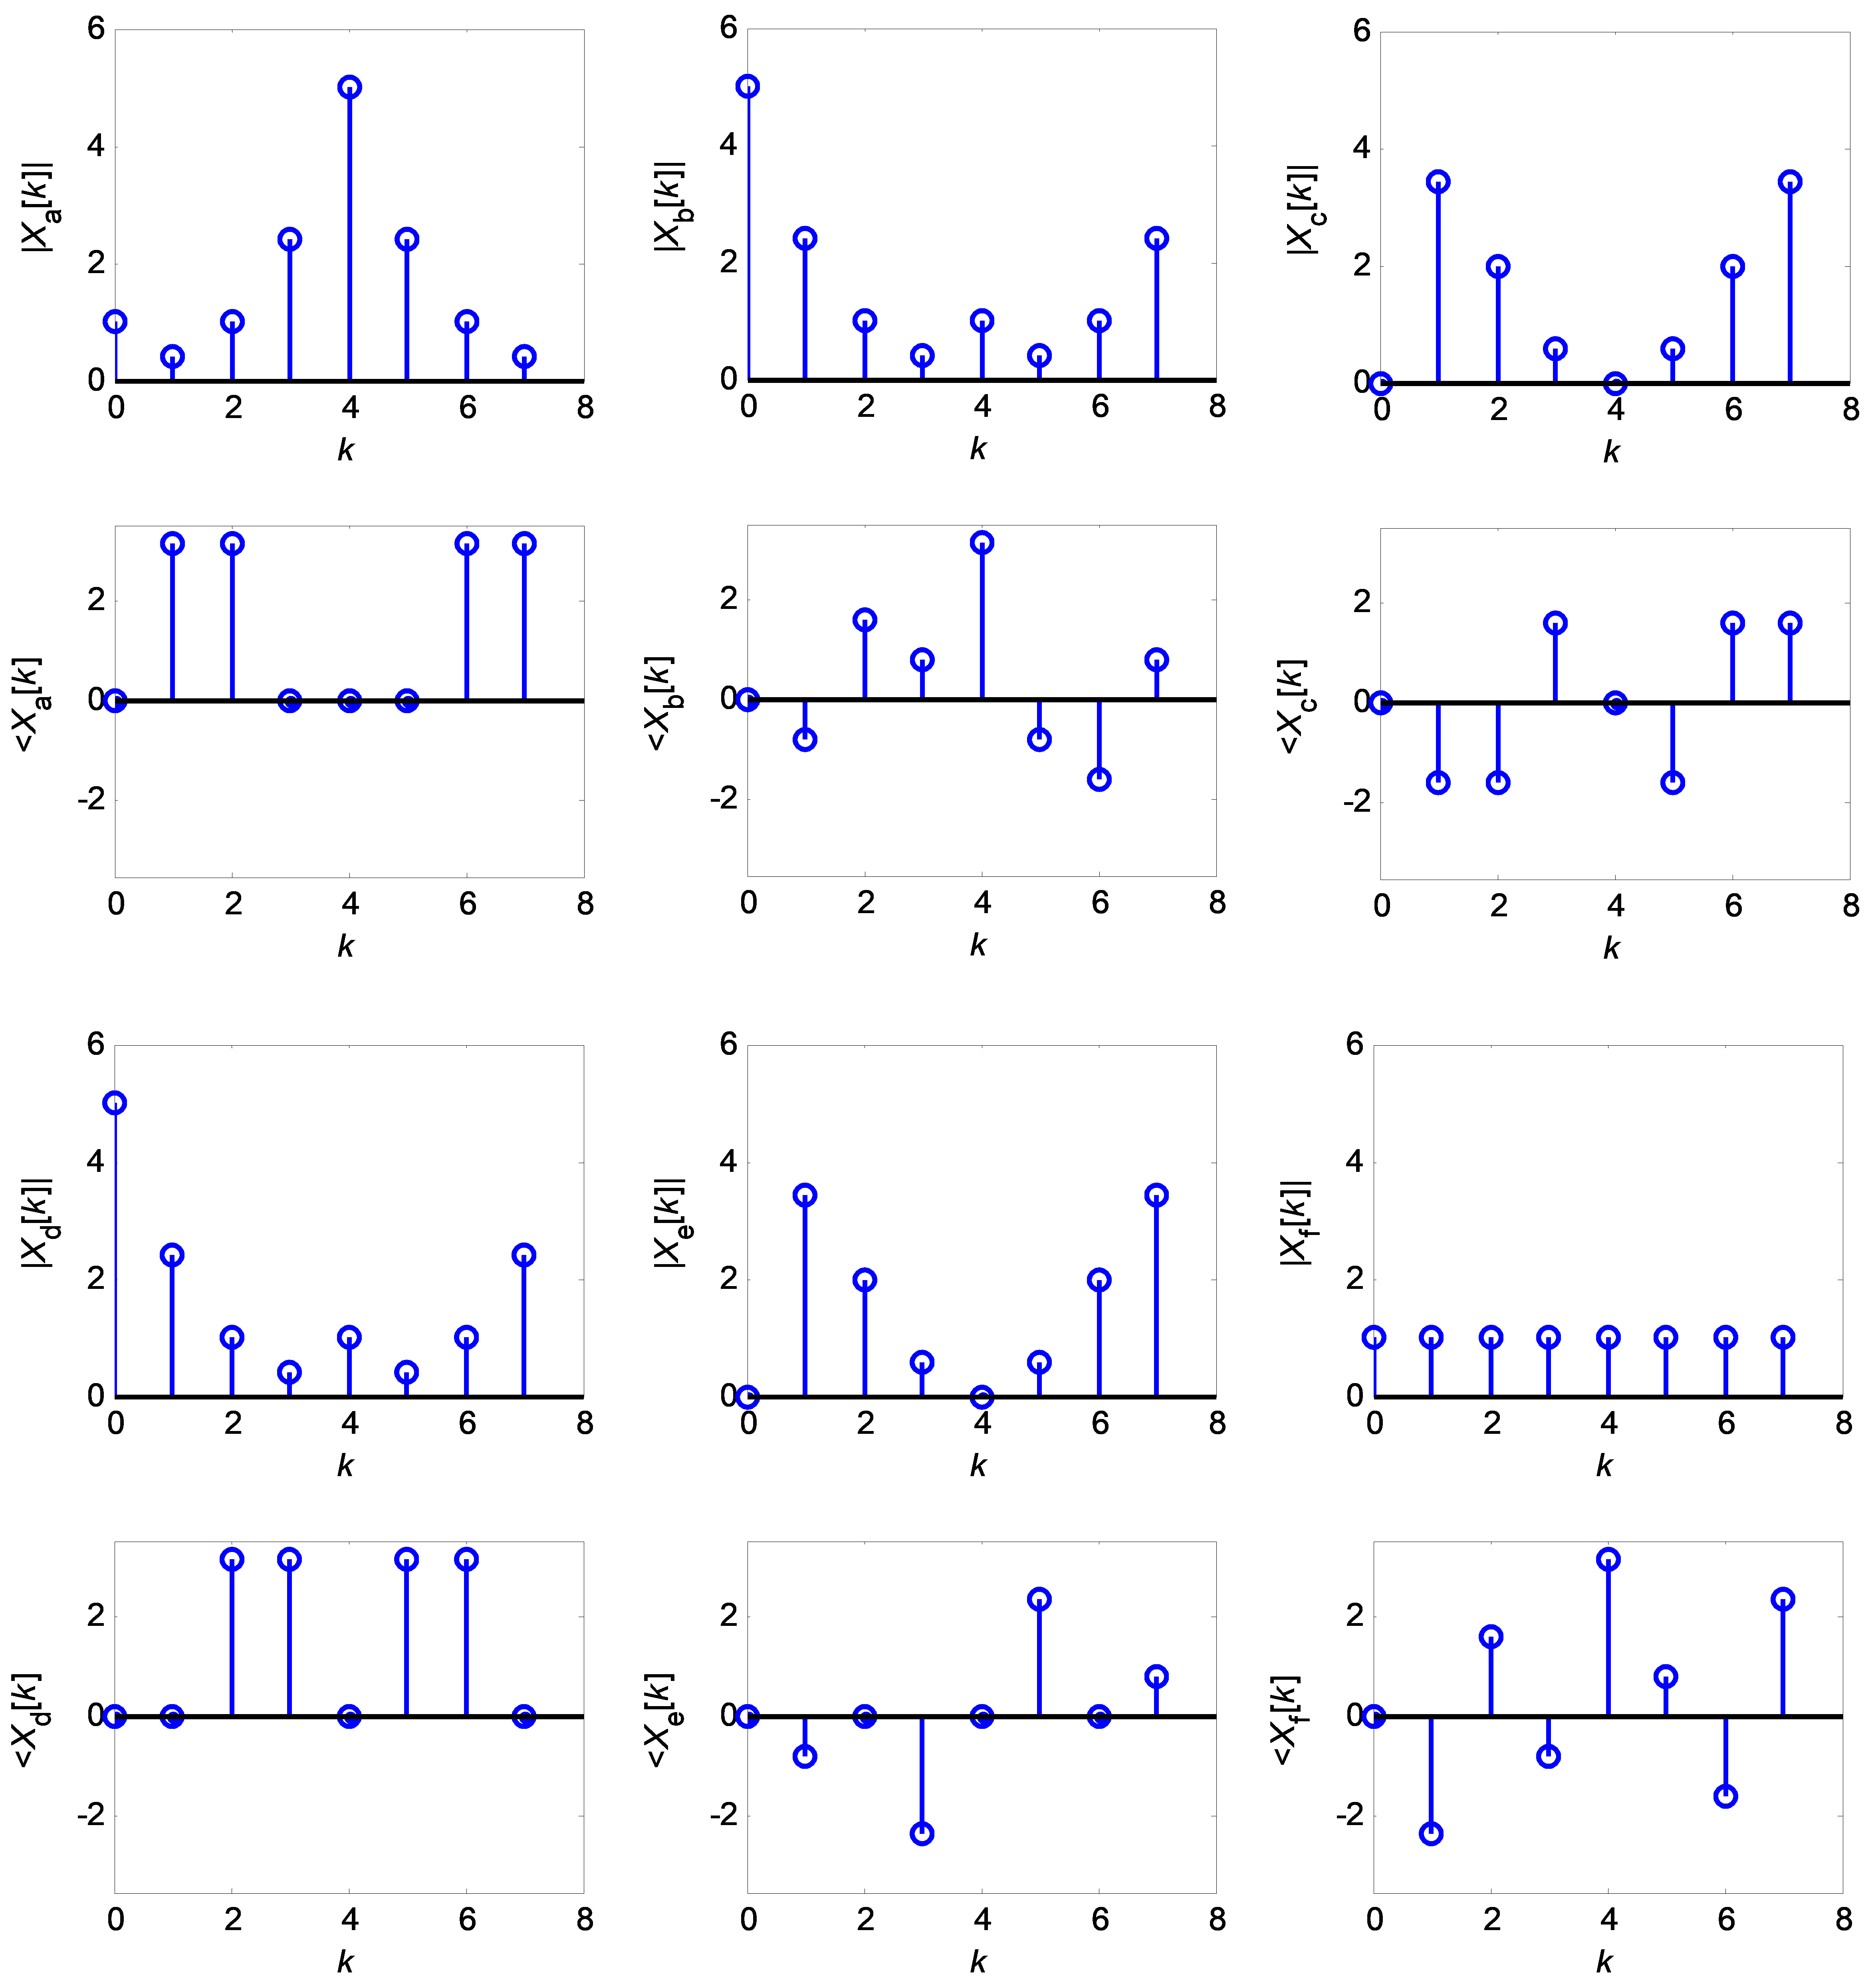
\includegraphics[width=\textwidth]{figs/dfts_mag.png}
	\caption{Magnitude ($|\cdot|$) and phase ($\angle \cdot$) of DFTs $X_a[k], \ldots, X_f[k]$}
	\label{fig:dfts}
\end{figure}
\FloatBarrier
 
~~~
 
\newpage
\noindent {\bf Problem 4: Linear convolution and circular convolution (20 points)} 

\begin{description}
	\item [(a)] Given a $L$-point sequence $x[n]$ and a $P$-point sequence $h[n]$, under what conditions would the $N$-point circular convolution match the linear convolution i.e, $x[n] \ast h[n] = x[n]~\encircle{N}~h[n]$?
	
	\item[(b)]  Several times during the course we used the Matlab function \texttt{xcorr} to estimate the autocorrelation or the cross-correlation function of signals. \underline{Without any normalization}, \texttt{xcorr} computes the the deterministic cross-correlation function, which can be expressed as a linear convolution:
	\begin{equation}
		c_{xy}[m] = \sum_{l = -\infty}^{\infty} x[m+l]y^*[l] = x[m]\ast y^*[-m]
	\end{equation}
	
	Assuming that both $x[m]$ and $y[m]$ are $L$-point sequences ($x[m] = 0, m < 0$ or $m \geq L$ and $y[m] = 0, m < 0$ or $m \geq L$), propose a method of calculating $c_{xy}[m]$ using FFTs and IFFTs. Give an equation for $c_{xy}[m]$ using your method and specify the length $N$ of the FFTs/IFFTs involved.
	
	\noindent\textit{Hint:} Don't forget to use the conjugate and time reversal properties of the DFT.
	
	\noindent\textit{Note:} If you want to test your method numerically, remember that according to the FFT/IFFT convention, your answer will be indexed from $0$ up to $N-1$. However, $c_{xy}[m]$ is defined from $-(N-1)/2$ up to $(N-1)/2$. Hence, you should use the command \texttt{fftshift} to match your method with the output of \texttt{xcorr}. Answers with and without \texttt{fftshift} will be accepted.
	
	\item [(c)] How would your method be simplified if instead of the cross-correlation function, we were calculating the autocorrelation function i.e., $y[n] = x[n]$?
\end{description}

\newpage
\noindent {\bf Problem 5: Overlap-add or overlap-save? (25 points + 10 points extra)} 

\begin{description}
	\item[(a)] Use either the overlap and add or overlap and save method to implement the notch FIR filter you designed in Homework \#5 to filter out the 60 Hz interference of the ECG signal. On the same graph plot the outcome of your implementation, the result of filtering with the function \texttt{filter}, and the ``clean'' ECG signal. Specify the block length $L$ and the FFT size $N$ that you chose in your implementation. You may want to read parts (b) and (c) before choosing these values. 
	
	\noindent\textit{Note:} It is not important for this question whether you designed a good notch filter or not. If you prefer, you can also use the FIR filter provided in the solutions of Homework \#5. However, the main point of this question is to understand the implementation of block convolution through overlap and add or overlap and save methods.
	
	\item [(b)] Compare the number of multiplications of your method with a direct implementation of an FIR filter. For this comparison, use the following metric
	\begin{equation}
		C = \frac{\text{\# of multiplications}}{\text{\# of useful output samples}}.
	\end{equation} 
	
	According to this metric, a direct implementation of an FIR filter of order $M = 52$ has complexity $C = 53$, since it requires 53 multiplications per each useful output sample. On the other hand, each FFT requires $\approx 2N(\log_2N-1)$ multiplications, but remember that not all $N$ outputs are useful in the overlap and add or overlap and save methods.
	
	\noindent\textit{Note:} Don't be surprise if the number of operations required by block convolution isn't much smaller than the direct FIR filter. This filter is not long enough for the FFT to yield significant savings in computation.
	
	\item [(c)] Give an expression for $C$ in terms of the filter order $M$ and the FFT length $N$. This equation should not depend on whether you chose overlap and add or overlap and save. On a single graph, plot $C$ as a function of $N$ when $M = 50$, $M = 100$, and $M = 150$. To facilitate visualization, for each value of $M$, plot $C$ using $N$ in a range from $2M$ up to 5000. For simplicity, your plot may include non-integer values of $N$.
	
	\noindent\textit{Note:} This exercise should show you that for each filter order $M$ there is an \underline{optimal} FFT size $N$. The optimal block size $L$ then follows from knowing $N$ and $M$.
		
	\item[(d) Optional] (extra 10 points) Implement the other method that you did not implement in part (a).
\end{description}


\newpage
\noindent {\bf Problem 6: Spectrograms (Question 10.32 of the textbook) (15 points)} 

An analog signal consisting of a sum of sinusoids was sampled with sampling rate of $f_s = 10000$ samples/s to obtain $x[n] = x_c(nT)$. Four spectrograms showing the time-dependent Fourier transform $|X[n, \lambda)|$ were computed using either a rectangular window or Hamming window. They are plotted in the figure below. 
\vspace{-0.3cm}
\begin{figure}[h!]
	\centering
	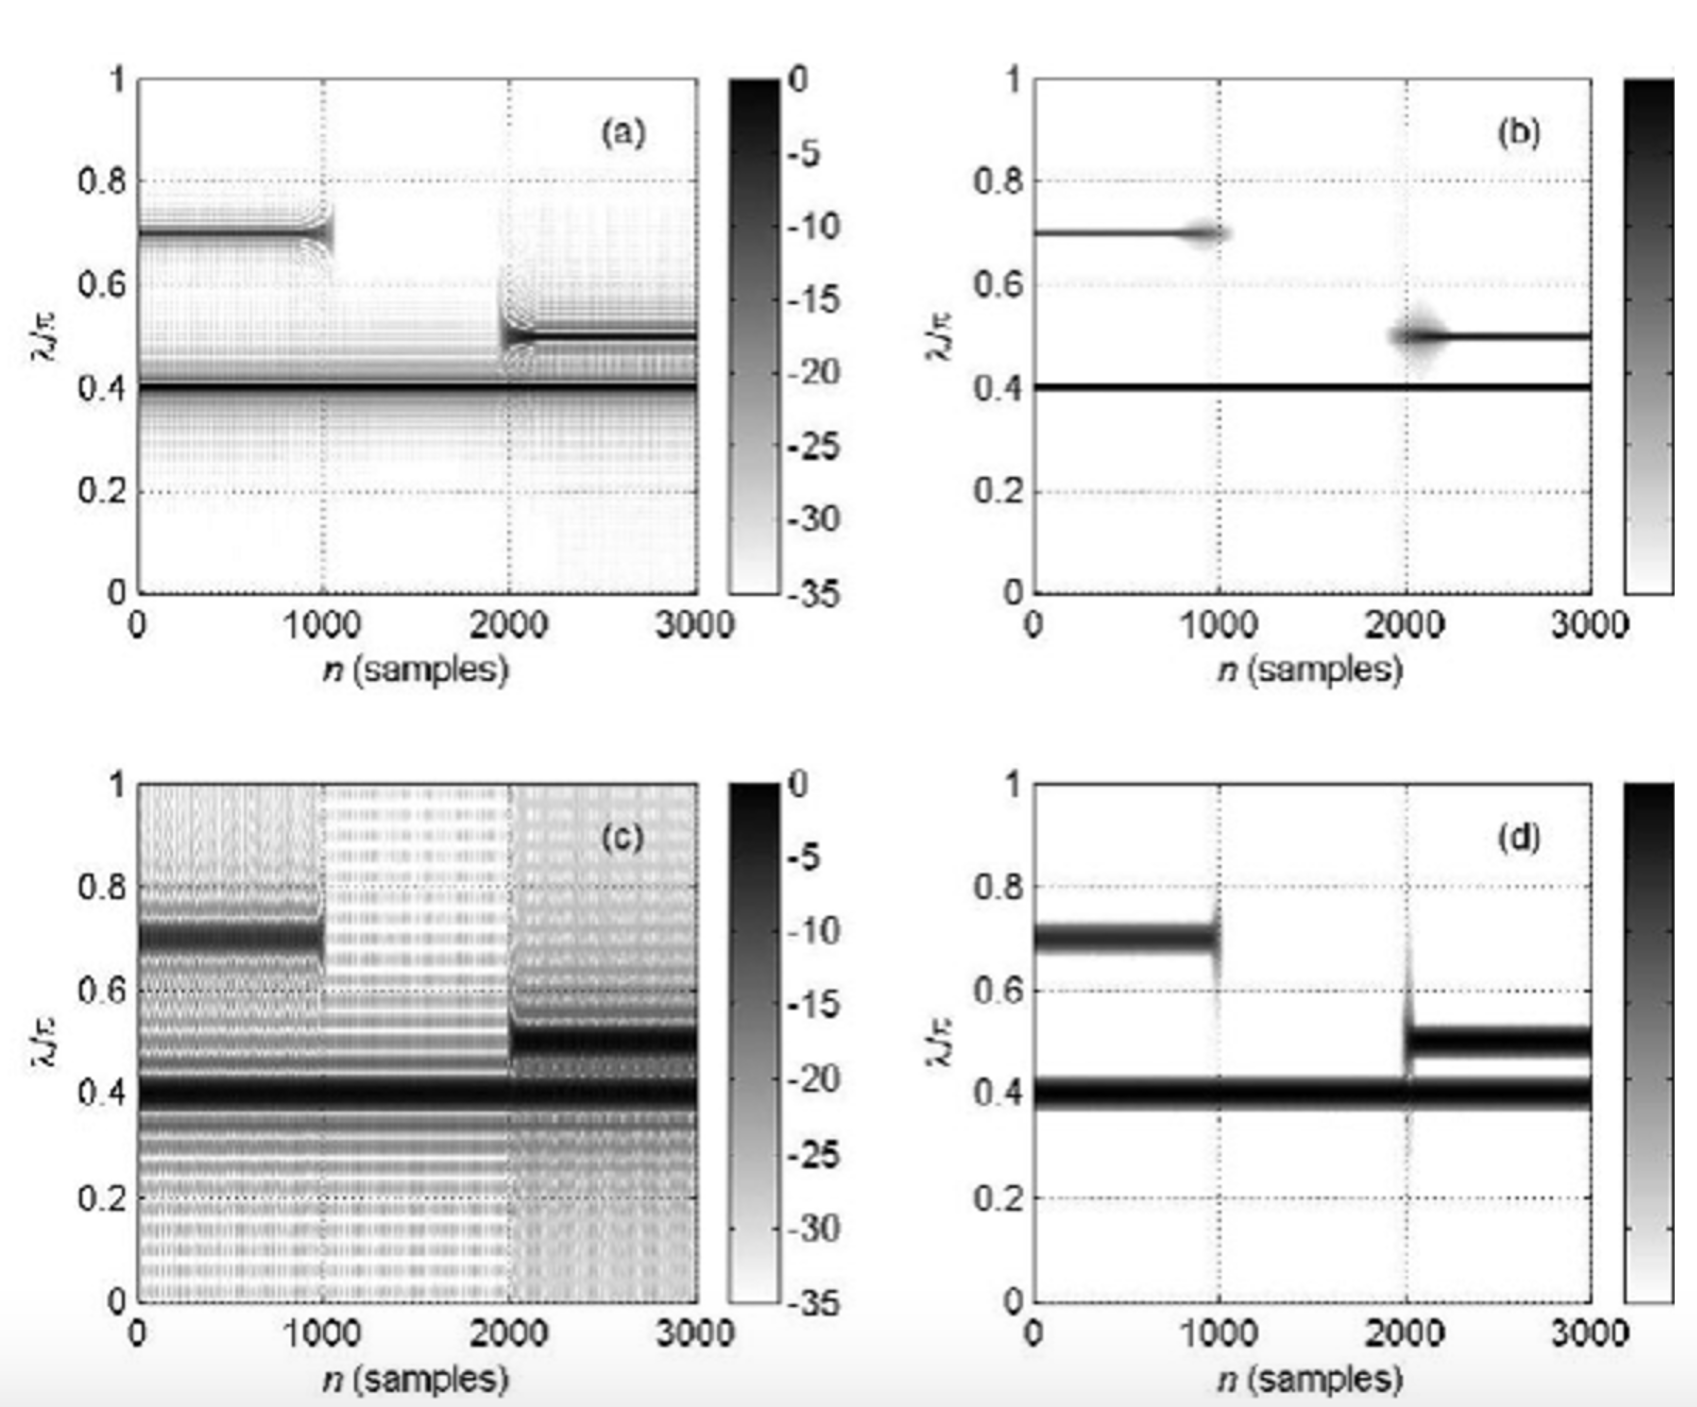
\includegraphics[width=0.9\textwidth]{figs/spectrograms.png}
	\caption{Spectrograms of $|X[n, \lambda)|$. The $y$-axis of all spectrograms is $\lambda/\pi$. The magnitude of the spectrograms is plotted in log scale and only the top 35 dB is shown.}
\end{figure}

Answer the following questions and give a brief justification to support your answers. 
\begin{description}
	\item[(a)] Which spectrograms were computed with a rectangular window?
	
	\begin{tabular}{cccc}
		(a) & (b) & (c) & (d)
	\end{tabular}
	
	\item[(b)] Which pair or pairs of spectrograms have approximately the same frequency resolution?
	
	\begin{tabular}{ccccc}
		(a\&b) & (b\&d) & (c\&d) & (a\&d) & (b\&c)
	\end{tabular}
	
	\item[(c)] Which spectrogram has the shortest time window?
	
	\begin{tabular}{cccc}
		(a) & (b) & (c) & (d)
	\end{tabular}
	
	\item[(d)] Write an equation for the continuous-time signal $x_c(t)$ that when sampled at sampling rate of $f_s = 10000$ samples/s would produce the above spectrograms. Be complete as you can in your description of the signal and indicate any parameters that cannot be obtained from the spectrograms.
\end{description}

\newpage
\noindent {\bf Problem 7: Frequency modulation (FM) (extra 20 points)}
 
A frequency-modulated signal with sinusoidal modulation is defined by the equation
\begin{equation} \label{eq:fm-signal}
	x_{FM}(t) = \cos(\theta(t)) = \cos(\Omega_ct + \beta\sin(\Omega_m t)),
\end{equation}
where $\Omega_c$ is the carrier frequency, $\Omega_m$ is the modulating frequency, and $\beta$ is called the modulation index. In FM transmission, as in radios, the modulating frequency $\Omega_m$ is changed according to the signal being transmitted e.g., a song.

\begin{description}
	\item[(a)] Write an equation for the instantaneous (radian) frequency defined by
	\begin{equation}
		\Omega_i(t) = \dfrac{d\theta(t)}{dt}.
	\end{equation}
	
	Why is the quantity $\beta\Omega_m$ called the maximum frequency deviation? For frequencies $\Omega_c = 2\pi(1000)$ and $\Omega_m = 2\pi$, either sketch or plot $\Omega_i(t)/(2\pi)$ for $0 \leq t \leq 4$ seconds, for $\beta = 0.2$ and for $\beta = 500$.
	
	\item[(b)] Show that if $\beta << \pi/2$, we can approximate $x_{FM}(t)$ as
	\begin{equation}
		x_{FM}(t) \approx \cos(\Omega_ct) - \beta\sin(\Omega_mt)\sin(\Omega_ct)
	\end{equation}
	This is called the \textit{narrowband FM approximation}. Either write an equation or a description of the Fourier transform $X_{FM}(j\Omega) = \mathcal{F}\{x_{FM}(t)\}$. Your description could be something like ``there will be impulses at frequencies...''.
	
	\item[(c)] The FM signal in \eqref{eq:fm-signal} with $\Omega_c = 2\pi(1000)$, $\Omega = 2\pi$ is sampled with a sampling rate of $F_s =1/T =8000$ samples/s. Give an equation, leaving $\beta$ as a parameter for the samples $x[n] = x_{FM}(nT)$.
	
	\item[(d)] In Matlab, generate 32768 samples of the FM signal in part (c) for the case $\beta = 0.2$. Listen to the signal using the function \texttt{soundsc()}.
	\begin{description}
		\item[(i)] Compute a single 32768-point DFT of the signal (use a rectangular window). Make a plot of the DFT magnitude. Label the frequency axis in terms of analog frequencies: $-Fs/2 \leq F \leq Fs/2$ in Hz. 
		
		\textit{Note:} It will be helpful to use the command \texttt{axis([990 1010 0 0.5])} to look only at the frequencies in the band
		$990 \leq F \leq 1010$ Hz. Is what you see consistent with your answer to part (b)? 
		
		\item[(ii)] Use the Matlab function \texttt{spectrogram} to plot the spectrogram of the sampled FM signal. Use a Hamming window of length 256 with overlap of 250 samples. Does your spectrogram show the variation of instantaneous frequency that you plotted in part (a)? If not, why not?
	\end{description}

	\item[(e)] Now generate 32768 samples of the FM signal in part (c) for the case $\beta = 500$. Listen to the signal using the function \texttt{soundsc()}.
	\begin{description}
		\item[(i)] Compute a single 32768-point DFT of the signal (use a rectangular window). Make a plot of the DFT magnitude. Label the frequency axis in terms of analog frequencies: $-Fs/2 \leq F \leq Fs/2$ in Hz. 

		\item[(ii)] Use the Matlab function \texttt{spectrogram} to plot the spectrogram of the sampled FM signal. Use a Hamming window of length 256 with overlap of 250 samples. Does your spectrogram show the variation of instantaneous frequency that you plotted in part (a)? 
		
		\item[(iii)] Experiment with window length and overlap to see how these parameters affect the image. Specifically, take a look at windows that are much shorter and also much longer than 256. How would the choice of window length depend upon the frequencies $\Omega_c$ and $\Omega_m$ if we wish to track the time variation of the instantaneous frequency with good resolution?
	\end{description}

\end{description}
\end{document}
